\subsection{Fundamentals, Purpose}

\begin{frame}
	\frametitle{Introduction: LTI Filters}
%	\framesubtitle{LTI Filters}
	Signal: temporal variable $x(k)$ with $\{x(k)\}_{k \geq 0} \in \mathbb{R}$
	\begin{figure}
	\begin{tikzpicture}[domain=0:7.5, samples=1000]
		\draw[->] (-0.2,0) -- (10.2,0) node[right] {\tiny$k$};
		\draw[->] (0,-1.2) -- (0,7.2) node[above] {};
		\draw[color=blue] plot[id=sin] function{sin(x)+sin(2*x)+sin(3*x)+sin(4*x)+sin(5*x)+sin(6*x)+sin(7*x) * sin(8*x) +sin(9*x) *sin(10*x)} node[right] {\tiny$u(k)$};
		\draw (3.8cm,-0.3cm) -- (5.8cm,-0.3cm) [->, thick] node[above,near end]{};
		\draw (0.3cm,-0.3cm) -- (2.3cm,-0.3cm) [->, thick] node[above,near end]{};
		\draw (2.3cm,-0.8cm) rectangle ++ (1.5cm,1cm)[thick] node [midway]{$\mathcal{H}$}; 
		\draw[->] (23.8,0) -- (33.8,0) node[right] {\tiny$k$};
		\draw[->] (24,-1.2) -- (24,7.2) node[above] {};
		\draw[color=red, xshift=117] plot[id=out] function{2*sin(x)} node[right] {\tiny$y(k)$};
	\end{tikzpicture}
	\end{figure}

	LTI (Linear Time Invariant) filters are particular filters that are:
	\begin{itemize}
		\item Linear: outputs are linear combinations of inputs (allows to use linear algebra definitions)
		\item Time-Invariant: all coefficients are constant
	\end{itemize}

	
\end{frame}

\begin{frame}
	\frametitle{Purpose of this work}
%	What is the purpose of this work?
	\begin{itemize}
		\item Lopez's PhD thesis studies how to compute LTI filters in software:
			\begin{itemize} 
				\item scheduling issues
				\item fixed size
			\end{itemize} 
		\item The goal here is to do such a work in hardware, where we have more flexibility:
			\begin{itemize} 
				\item full parallelism
				\item arbitrary size
			\end{itemize} 
	\end{itemize}
	In this context, constraints become degrees of freedom.
\end{frame}

\subsection{FIR, IIR}
\begin{frame}
	\frametitle{FIR, IIR}
	\only<1,2,3> {The most simple LTI Filter: the FIR (Finite Impulse Response) filter}
	\only<4-> {Full LTI complexity: the IIR (Infinite Impulse Response) filter:}
	\begin{equation} \label{iirdef}
		\only<1,2,3>{y(k)=\sum_{i=0}^n b_i u(k-i)}
		\only<4->{y(k)=\sum_{i=0}^n b_i u(k-i) - \sum_{i=0}^n a_i y(k-i)}
	\end{equation}


\only<2,3->{Abstract architecture for the direct form realization of \only<2,3>{a FIR}\only<4->{an IIR} filter:}
	\only<2->{
\begin{figure}[]
\resizebox{!}{100pt}{
  \begin{tikzpicture}
	\only<4>{
     \draw[dotted,green, fill=green!20] (-5ex,-3.5ex) rectangle +(61ex,-15ex);   
	}
	\only<4->{
     \node[green!50!black]  at (-2ex,-17.5ex) {{\small SOPC}};   
	}
	\only<3,5->{
	\node[draw, thick, dotted, rectangle, minimum width = 6cm, minimum height=2.9cm, align=left, green!100, fill=green!20] (sop1) at (2cm,-2.1cm) {};
	}
	\only<5->{
	\node[draw, thick, dotted, rectangle, minimum width = 4cm, minimum height=2.9cm, align=left, green!100, fill=green!20] (sop2) at (7.5cm,-2.1cm) {};
	}
    \draw[hwbus] (-8, 0) node[left] {$u(k)$} --  ++(8, 0)  ;
    \draw[hwbus,->] (-8, 0) --  ++(3, 0); % just for the arrow
    \foreach \i in {0,...,3} {
      \draw[hwbus, ->] ($(8*\i, 0)$) --  ++(0, -5);
      \draw[hwblock] ($(8*\i, -5)$) -- ++(3, 0) -- ++(-3, -4) -- ++(-3, 4) -- cycle; 
      \node (n) at ($(8*\i , -6.5)$)  {$b_{\i}$} ;
%      \draw ($(8*\i  + 0.5, -11)$) node[left,tt=black!50] {\footnotesize $p_b(k,\i)$} ;
%      \draw ($(8*\i  - 0.2, -11)$) node[right,text=black!50] {\footnotesize $p_b(k,\i)$} ;

%      \draw[hwbus, ->] ($(8*\i ex, 0ex)$) --  ++(0, -5ex);
    }

    
    \draw[hwbus] (0, -9) -- ++(0,-6);
      \coordinate (n) at  (0,-15);
    \foreach \i in {1,...,3} {
      \draw[line width=3pt] ($(8*\i  - 4, -3)$) --  +(0, 6);
      \draw[hwbus] ($(8*\i  - 8, 0)$) --  +(8,0) node [above,text=blue] {\footnotesize $u(k-\i)$};
      \draw[hwbus,->] ($(8*\i  - 8, 0)$) --  ++(3, 0); % just for the arrow
      % The adders 
      \coordinate (nm1) at  (n.east);
      \draw ($(8*\i , -15)$) node[hwblock,circle,minimum height=3] (n) {$+$};
      \draw[hwbus, ->]  ($(8*\i , -9)$) -- (n.north);
      \draw[hwbus, ->]  (nm1) -- (n.west);
      \draw[hwbus]  (n.east) -- ++ (3,0);
    }
	\only<6>{\node [] at (30,-15) {/};}

    %\draw (74, -15) node[hwblock,align=center] (fr) {final\\round} ;

	\only<4->{
    \foreach \i in {1,...,3} {
      \draw[hwbus, ->] ($(-8*\i  + 60 , 0)$) --  ++(0, -5);
      \draw[hwblock] ($(-8*\i  + 60 , -5)$) -- ++(3, 0) -- ++(-3, -4) -- ++(-3, 4) -- cycle; 
      \node (ai) at ($(-8*\i  + 60 , -6.5)$)  {$a_{\i}$} ;
      %\draw ($(-8*\i  +60 + 0.5, -11)$) node[left,text=black!50] {\footnotesize $p_a(k,\i)$} ;
      %\draw ($(-8*\i  +60 - 0.2, -11)$) node[right,text=black!50] {\footnotesize $p_a(k,\i)$} ;
      \draw ($(-8*\i  + 60 , -15)$) node[hwblock,circle,minimum height=3] (n) {$+$};
      \draw (n.north) node[left]{\bf -};
      \draw[hwbus, ->] ($(-8*\i  + 60, -9)$) --  (n.north);
      \draw[hwbus, <-] (n.west) -- ++(-5,0);
      % The registers
      \draw[hwbus] ($(-8*\i  + 60  +8, 0)$) --  ++(-8, 0) node [above,text=blue] {\footnotesize $y\only<6>{^*}(k-\i)$};
      \draw[hwbus,->] ($(-8*\i  + 60  +8, 0)$) --  ++(-3, 0); % just for the arrow
      \draw[line width=3pt] ($(-8*\i  +60 + 4, -3)$) --  +(0, 6);
    }
	}
    \only<2,3>{\draw[hwbus, <-] (40,-15) -- ++(-10,0) node [near end,xshift=-5mm] {\only<6>{/}} node [near end,below, text width=4cm, xshift=0.5cm] {\only<4>{\footnotesize$(msb_{out},$ $ lsb_{out}+g)$}} node[near start,above] {\only<2,3>{$y(k)$}} -- ++(-1,0) ;
	}
    \only<4->{\draw[hwbus, <-] (70,-15) -- ++(-15,0) node [near end] {\only<6>{/}} node [near end,below, text width=4cm, xshift=1.5cm] {\only<6>{\footnotesize$(msb_{out},$ $ lsb_{out})$}} node[near start,above] {$y\only<6>{^*}(k)$} -- ++(-1,0) ;
	}
    %\draw[hwbus, ->] (fr.east) -- ++(12,0) node [midway] {/} node [midway,below, text width=2cm] {\footnotesize$(msb_{out},$ $lsb_{out}+g)$} node[right] {$\yout(k)$} ;
	\only<4->{
    \draw[hwbus] ($(60 , 0)$) --  ++(0,-15);
    \draw[hwbus,<-] ($(60 , -5)$) --  ++(0,-5);
	}
	\only<2->{
     \node[green!50!black]  at (-0.5cm,-4cm) {};% node for keeping scale
	}
	\only<3,5->{
     \node[green!50!black]  at (-0.5cm,-3.4cm) {{\small SOPC}};   
	}

	\only<5->{
     \node[green!50!black]  at (6.0cm,-3.4cm) {{\small SOPC}};   
	}


  \end{tikzpicture}
  }
\only<3->{
	\\
SOPC (Sum Of Products by Constants):\\basic block of LTI filters implementation.
}

%\caption{Abstract architecture for the direct form realization of an LTI filter \label{fig:ltiarch}}

\end{figure}
	}
\end{frame}

%\begin{frame}
%	Here we have loop-backs, so registers:\\
%		\begin{center}
%	Loop-backs $\iff$ Registers
%		\end{center}
%	We can generalise by introducing state registers.
%\end{frame}

\subsection{State-Space representation}
\begin{frame}
	\frametitle{State-Space representation}
	Let's define $\boldsymbol{x}(k)$ a state vector (hardware register)
	\frametitle{State-Space representation}
	\framesubtitle{The ``ABCD" form}
	\begin{equation} \label{abcddef}
		\begin{cases}
			\boldsymbol{x}(k+1)= \boldsymbol{Ax}(k) + \boldsymbol{Bu}(k) \\
			\boldsymbol{y}(k+1)= \boldsymbol{Cx}(k) + \boldsymbol{Du}(k)
		\end{cases}
	\end{equation}
	\\
	With: \\
		\begin{center}
	$\boldsymbol{A} \in \mathbb{R}^{n_x \times n_x}$ ,
	$\boldsymbol{B} \in \mathbb{R}^{n_x \times n_u}$ , \\
	$\boldsymbol{C} \in \mathbb{R}^{n_y \times n_x}$ ,
	$\boldsymbol{D} \in \mathbb{R}^{n_y \times n_u}$
		\end{center}

	Equivalent matrix formulation:
	
	\begin{equation} \label{abcdef}
		\begin{pmatrix}
			\boldsymbol{x} (k+1)  \\
			\boldsymbol{y} (k+1) 
		\end{pmatrix}
		=
		\begin{pmatrix}
			\boldsymbol{A} & \boldsymbol{B} \\
			\boldsymbol{C} & \boldsymbol{D} \\
		\end{pmatrix}
		\begin{pmatrix}
			\boldsymbol{x} (k)  \\
			\boldsymbol{u} (k) 
		\end{pmatrix}
	\end{equation}

\end{frame}

%\begin{frame}


%\end{frame}


\subsection{The SIF: a unified realization representation }

\begin{frame}
	\frametitle{The SIF: a unified realization representation}
	Problems with ABCD:
	\begin{itemize}
		\item this doesn't gives an explicit order in the operations
		\item the whole analysis on precisions has to be rebuilt for each new realization.
	\end{itemize}

	The SIF (Speciallized Implicit Form) generalizes the state-space.\\
	Addition: $\boldsymbol{t}(k)$ describes explicit intermediate computations:

	%\frametitle{Definition of the SIF}
	\begin{equation} \label{sifdef}
		\begin{pmatrix}
			\boldsymbol{J} & \boldsymbol{0} & \boldsymbol{0} \\
			\boldsymbol{-K} & \boldsymbol{I}_{n_x} & \boldsymbol{0} \\
			\boldsymbol{-L} & \boldsymbol{0} & \boldsymbol{I}_{n_y} 
		\end{pmatrix}
		\begin{pmatrix}
			\boldsymbol{t} (k+1)  \\
			\boldsymbol{x} (k+1)  \\
			\boldsymbol{y} (k) 
		\end{pmatrix}
		=
		\begin{pmatrix}
			\boldsymbol{0} & \boldsymbol{M} & \boldsymbol{N} \\
			\boldsymbol{0} & \boldsymbol{P} & \boldsymbol{Q} \\
			\boldsymbol{0} & \boldsymbol{R} & \boldsymbol{S} 
		\end{pmatrix}
		\begin{pmatrix}
			\boldsymbol{t} (k)  \\
			\boldsymbol{x} (k)  \\
			\boldsymbol{u} (k) 
		\end{pmatrix}
	\end{equation}
\begingroup

	\fontsize{7}{9}\selectfont
	$J$ is a lower triangular matrix with only ones on the diagonal.
\endgroup
%	\\
%	\vspace{10pt}
%	With: \\
%	\begin{eqnarray}
%		\boldsymbol{J} \in \mathbb{R}^{n_t \times n_t},\boldsymbol{M} \in \mathbb{R}^{n_t \times n_x},\boldsymbol{N} \in \mathbb{R}^{n_t \times n_u}, \nonumber \\
%		\boldsymbol{K} \in \mathbb{R}^{n_x \times n_t},\boldsymbol{P} \in \mathbb{R}^{n_x \times n_x},\boldsymbol{Q} \in \mathbb{R}^{n_x \times n_u}, \\
%		\boldsymbol{L} \in \mathbb{R}^{n_y \times n_t},\boldsymbol{R} \in \mathbb{R}^{n_y \times n_x},\boldsymbol{S} \in \mathbb{R}^{n_y \times n_u}, \nonumber \\
%	\end{eqnarray}

\end{frame}

\begin{frame}
	\frametitle{Example}
	\begin{figure}
		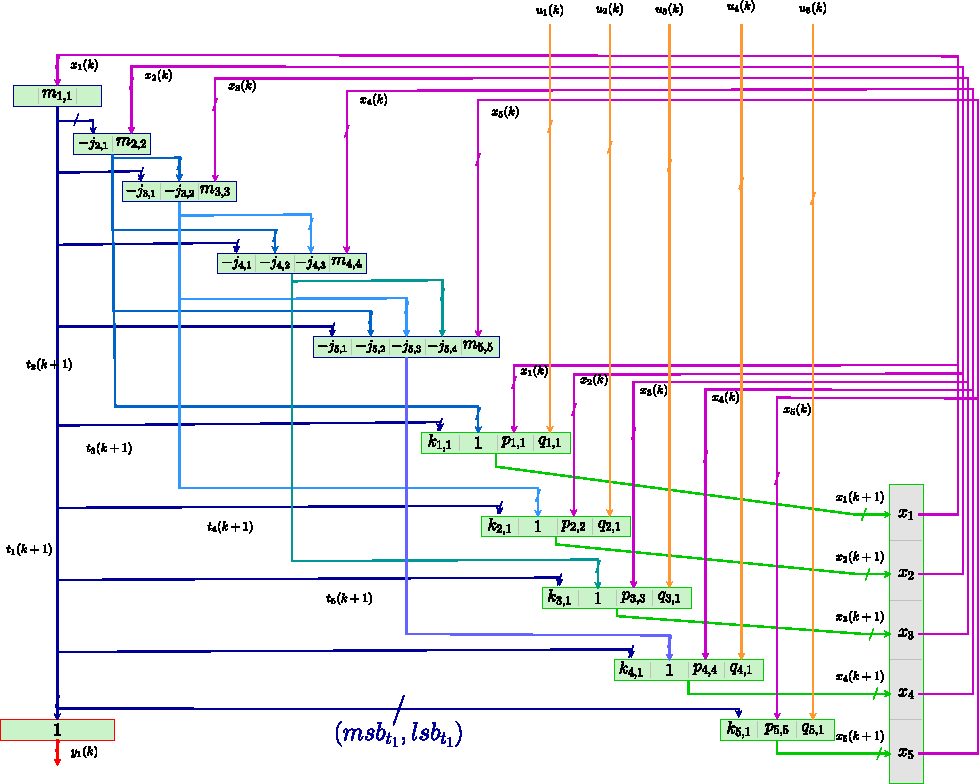
\includegraphics[scale=0.54]{pictures/exampleGreenScheme.pdf}
	\end{figure}
\end{frame}

%\begin{frame}
%	\frametitle{The SIF as an algorithm} %TODO: put just before the example. put arch design instead
%	\begin{algorithm}[H]
%		\For{int i = 0 ; $i \leq n_t$; i++}{
%			$\boldsymbol{t}_i(k+1) \leftarrow - \sum\limits\limits_{j<i} \boldsymbol{J}_{ij}\boldsymbol{t}_j(k+1) + \sum\limits_{j=1}^{n_x} \boldsymbol{M}_{ij}\boldsymbol{x}_j(k) + \sum\limits_{j=1}^{n_u} \boldsymbol{N}_{ij}\boldsymbol{u}_j(k)$
%		}
%		\For{int i = 0 ; $i \leq n_x$; i++}{
%			$\boldsymbol{x}_i(k+1) \leftarrow \sum\limits_{j=1}^{n_t} \boldsymbol{K}_{ij}\boldsymbol{t}_j(k+1) + \sum\limits_{j=1}^{n_x} \boldsymbol{P}_{ij}\boldsymbol{x}_j(k) + \sum\limits_{j=1}^{n_u} \boldsymbol{Q}_{ij}\boldsymbol{u}_j(k)$
%		}
%		\For{int i = 0 ; $i \leq ny$; i++}{
%			$\boldsymbol{y}_i(k) \leftarrow \sum\limits_{j=1}^{n_t} \boldsymbol{L}_{ij}\boldsymbol{t}_j(k+1) + \sum\limits_{j=1}^{n_x} \boldsymbol{R}_{ij}\boldsymbol{x}_j(k) + \sum\limits_{j=1}^{n_u} \boldsymbol{S}_{ij}\boldsymbol{u}_j(k)$
%		}
%		\caption{Computation of SIF outputs from inputs}
%	\end{algorithm}
%\end{frame}

%\begin{frame}
%	\frametitle{A more common notation} %TODO: backup
%	A non-compact notation:
%	\begin{equation} \label{sifdef}
%		\begin{pmatrix}
%			\boldsymbol{J} & \boldsymbol{0} & \boldsymbol{0} \\
%			\boldsymbol{-K} & \boldsymbol{I}_{n_x} & \boldsymbol{0} \\
%			\boldsymbol{-L} & \boldsymbol{0} & \boldsymbol{I}_{n_y} 
%		\end{pmatrix}
%		\begin{pmatrix}
%			\boldsymbol{t} (k+1)  \\
%			\boldsymbol{x} (k+1)  \\
%			\boldsymbol{y} (k) 
%		\end{pmatrix}
%		=
%		\begin{pmatrix}
%			\boldsymbol{0} & \boldsymbol{M} & \boldsymbol{N} \\
%			\boldsymbol{0} & \boldsymbol{P} & \boldsymbol{Q} \\
%			\boldsymbol{0} & \boldsymbol{R} & \boldsymbol{S} 
%		\end{pmatrix}
%		\begin{pmatrix}
%			\boldsymbol{t} (k)  \\
%			\boldsymbol{x} (k)  \\
%			\boldsymbol{u} (k) 
%		\end{pmatrix}
%	\end{equation}
%	An easier way to communicate SIFs:\\
%		The Z matrix:\\
%	\begin{equation}
%		Z = 
%		\begin{pmatrix}
%			\boldsymbol{-J} & \boldsymbol{M} & \boldsymbol{N} \\
%			\boldsymbol{K} & \boldsymbol{P} & \boldsymbol{Q} \\
%			\boldsymbol{L} & \boldsymbol{R} & \boldsymbol{S} 
%		\end{pmatrix}
%	\end{equation}
%\end{frame}

\begin{frame}
	\frametitle{Workflow}

		\begin{figure}[h] 

		\resizebox{300pt}{!}{
		  \tiny
		  \begin{tikzpicture}[]
		  
%		   \node[draw, fill = orange!20, shape = rectangle, minimum width = 2cm, minimum height= 2cm] at (-4cm,4cm) {FixSIF} ;
%		   \node[draw, fill = gray!20, shape = rectangle, minimum width = 1cm, minimum height= 1.2cm] at (-1cm,4cm) {VHDL} ;
%			\draw (-6.5cm, 4.5cm) -- (-5cm,4.5cm) [->, thick] node[above,near start, text width = 3cm, align=center, xshift=-1cm]{$(a_i)_{1 < \leq i \leq n},(b_i)_{1 < \leq i \leq n}$};
%			\draw (-6.5cm, 4cm) -- (-5cm,4cm) [->, thick] node[above,near start, text width = 3cm, align=center, xshift=-1cm]{input format ($msbs_u$,$lsbs_u$)};
%			\draw (-6.5cm, 3.5cm) -- (-5cm,3.5cm) [->, thick] node[above,near start, text width = 3cm, align=center, xshift=-1cm]{output accuracy ($msbs_y$,$lsbs_y$)};
%
%			\draw (-3cm, 4cm) -- (-1.5cm,4cm) [->, thick] node[above,near start, text width = 3cm, align=center, xshift=-1cm]{};
%			%zoom links
%			\draw (-5cm, 3cm) -- (-8.5cm,1.5cm) [-, thick, black!40] node[above,near start, text width = 3cm, align=center, xshift=-1cm]{};
%			\draw (-3cm, 3cm) -- (0.5cm,1.5cm) [-, thick, black!40] node[above,near start, text width = 3cm, align=center, xshift=-1cm]{};

			%zoom view
			%\draw (-9.5cm, 0.7cm) -- (-8cm,0.7cm) [->, thick] node[above,near start, text width = 3cm, align=center]{User filter specification};
			\draw (-5.5cm, 0.7cm) -- (-3.0cm,0.7cm) [->, thick] node[below,xshift=-1.2cm]{$\begin{pmatrix}\boldsymbol{-J} & \boldsymbol{M} & \boldsymbol{N} \\ \boldsymbol{K} & \boldsymbol{P} & \boldsymbol{Q} \\ \boldsymbol{L} & \boldsymbol{R} & \boldsymbol{S} \end{pmatrix}$};
			\draw[fill=orange!20] (-8cm,0.0cm) rectangle ++(2.5cm,1.4cm)[thick] node [midway, text width = 4cm, align=center]{Realization choice \\ by \\ Hilaire, Volkova  \\ team PEQUAN, LIP6 \\(Front-End)}; 
			\draw[fill=orange!20] (-3.0cm,0.0cm) rectangle ++(3.0cm,1.4cm)[thick] node [midway, text width = 3cm, align=center]{Flopoco core generation \\ (this work) \\(Back-End)}; 

			\draw (1cm,0cm) rectangle ++(1.1cm,1.4cm)[thick, fill=gray!20] node [midway]{VHDL}; 
			\draw (0.0cm, 0.7cm) -- (1cm,0.7cm) [->, thick] node[above,near start]{};

			\draw (-5.5cm, 2.0cm) -- (-4.0 cm, 2.0cm) -- (-4.0cm,1.3cm) -- (-3.0cm,1.3cm) [->, thick] node[below,xshift=-3.8cm, yshift=1cm]{input format ($msbs_u$,$lsbs_u$)};
			\draw (-5.5cm, 1.7cm) -- (-5.0 cm, 1.7cm) -- (-5.0cm,1.0cm) -- (-3.0cm,1.0cm) [->, thick] node[below,xshift=-4cm, yshift=1cm]{output accuracy ($msbs_y$,$lsbs_y$)};
		  \end{tikzpicture}

		}
		\end{figure}
		\centering
		Workflow overview of tools usage
\end{frame}

